\documentclass[aspectratio=169]{beamer}
\usepackage{graphicx}
\usepackage{listings}
\usepackage{xcolor}
\usepackage{amsmath}
\usepackage{tikz}
\usetikzlibrary{arrows,shapes,positioning}

\usetheme{Madrid}
\usecolortheme{beaver}
% Add these font size adjustments after \usetheme{Madrid}

\usetheme{Madrid}
\usecolortheme{beaver}

% Global font size adjustments
\usepackage{lmodern}  % Better font scaling
\renewcommand{\tiny}{\fontsize{5}{6}\selectfont}
\renewcommand{\scriptsize}{\fontsize{6}{7}\selectfont}
\renewcommand{\footnotesize}{\fontsize{7}{8}\selectfont}
\renewcommand{\small}{\fontsize{8}{9}\selectfont}
\renewcommand{\normalsize}{\fontsize{9}{10}\selectfont}
\renewcommand{\large}{\fontsize{10}{12}\selectfont}
\renewcommand{\Large}{\fontsize{12}{14}\selectfont}
\renewcommand{\LARGE}{\fontsize{14}{17}\selectfont}
\renewcommand{\huge}{\fontsize{17}{22}\selectfont}
\renewcommand{\Huge}{\fontsize{20}{25}\selectfont}

% Reduce title and section font sizes
\setbeamerfont{title}{size=\Large}
\setbeamerfont{subtitle}{size=\large}
\setbeamerfont{author}{size=\normalsize}
\setbeamerfont{institute}{size=\small}
\setbeamerfont{date}{size=\small}
\setbeamerfont{frametitle}{size=\large}
\setbeamerfont{framesubtitle}{size=\normalsize}

% Reduce itemize and enumerate font sizes
\setbeamerfont{itemize/enumerate body}{size=\small}
\setbeamerfont{itemize/enumerate subbody}{size=\footnotesize}
\setbeamerfont{itemize/enumerate subsubbody}{size=\scriptsize}

% Make code even smaller
\lstset{
    language=Python,
    basicstyle=\scriptsize\ttfamily,  % Changed from \tiny to \scriptsize
    keywordstyle=\color{blue},
    commentstyle=\color{green!60!black},
    stringstyle=\color{red},
    showstringspaces=false,
    breaklines=true,
    frame=single,
    backgroundcolor=\color{gray!10}
}
\title{Bridging IMP and Probabilistic Programming: \\ A JAX/NumPyro Interface for Molecular Modeling}
\author{Your Name}
\institute{Your Institution}
\date{\today}

% Code styling
\lstset{
    language=Python,
    basicstyle=\tiny\ttfamily,
    keywordstyle=\color{blue},
    commentstyle=\color{green!60!black},
    stringstyle=\color{red},
    showstringspaces=false,
    breaklines=true,
    frame=single,
    backgroundcolor=\color{gray!10}
}

\begin{document}

\frame{\titlepage}

%% SLIDE 1: Overview and Motivation
\begin{frame}{Overview: IMP meets Probabilistic Programming}
\begin{columns}[T]
\begin{column}{0.5\textwidth}
\textbf{Traditional IMP Workflow:}
\begin{itemize}
    \item Build molecular system
    \item Define scoring functions/restraints
    \item Optimize using MCMC
\end{itemize}

\vspace{0.5cm}
\textbf{Our Approach:}
\begin{itemize}
    \item \alert{Bridge IMP with JAX/NumPyro}
    \item Enable advanced sampling (HMC)
    \item Better uncertainty quantification
    \item Explore broader conformational landscapes
\end{itemize}
\end{column}

\begin{column}{0.5\textwidth}
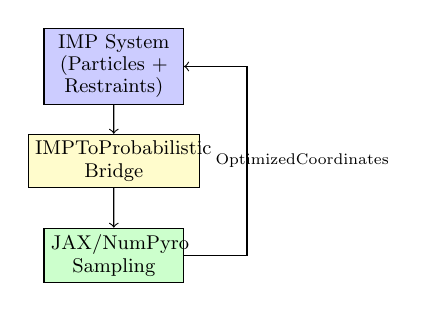
\begin{tikzpicture}[scale=0.8, transform shape]
    % IMP System
    \node[rectangle, draw, fill=blue!20, text width=2cm, text centered] (imp) at (0,3) {IMP System\\(Particles + Restraints)};
    
    % Bridge
    \node[rectangle, draw, fill=yellow!20, text width=2.5cm, text centered] (bridge) at (0,1.5) {IMPToProbabilistic\\Bridge};
    
    % NumPyro
    \node[rectangle, draw, fill=green!20, text width=2cm, text centered] (numpyro) at (0,0) {JAX/NumPyro\\Sampling};
    
    % Arrows
    \draw[->] (imp) -- (bridge);
    \draw[->] (bridge) -- (numpyro);
    \draw[->] (numpyro.east) -- ++(1,0) |- (imp.east);
    
    \node[right] at (1.5,1.5) {\footnotesize Optimized\\Coordinates};
\end{tikzpicture}
\end{column}
\end{columns}
\end{frame}

%% SLIDE 2: System Building and Data Extraction
\begin{frame}[fragile]{Step 1: IMP System Setup and Coordinate Extraction}
\begin{columns}[T]
\begin{column}{0.55\textwidth}
\textbf{IMP System Construction:}
\begin{lstlisting}
# Build multi-protein system
system = IMP.pmi.topology.System(model)
state = system.create_state()

# Create molecules with representations
molecule = state.create_molecule(
    name="protein_1", 
    sequence="AA",
    chain_id="A"
)
molecule.add_representation(
    resolutions=[1], 
    bead_ca_centers=True
)
\end{lstlisting}

\textbf{Coordinate Extraction:}
\begin{lstlisting}
def get_coordinates_array(self):
    coords = []
    for particle in self.particles:
        xyz = particle.get_coordinates()
        coords.append([xyz[0], xyz[1], xyz[2]])
    return np.array(coords)  # Shape: (N_particles, 3)
\end{lstlisting}
\end{column}

\begin{column}{0.45\textwidth}
\textbf{Key Concepts:}
\begin{itemize}
    \item \alert{NumPy Arrays}: Standard Python arrays
    \begin{itemize}
        \item Mutable, CPU-based
        \item Direct memory access
        \item Compatible with IMP's C++ backend
    \end{itemize}
    
    \vspace{0.3cm}
    \item \alert{JAX Arrays}: Functional programming arrays
    \begin{itemize}
        \item Immutable, JIT-compilable
        \item GPU/TPU compatible
        \item Automatic differentiation
    \end{itemize}
    
    \vspace{0.3cm}
    \item \alert{Array Conversion}: Critical bottleneck
    \begin{itemize}
        \item JAX → NumPy: \texttt{np.array(jax\_array)}
        \item Avoid in traced functions!
    \end{itemize}
\end{itemize}
\end{column}
\end{columns}
\end{frame}
\begin{frame}[t]{Slide 1: Key Differences (Part 1)}
\footnotesize
\begin{table}
\centering
\begin{tabular}{lcc}
\toprule
Aspect & NumPy Arrays & JAX Arrays \\
\midrule
Mutability & Mutable: Modify in-place (e.g., arr[0] = 10). & Immutable: Operations return new arrays; use .at[idx].set(). \\
Hardware Support & Primarily CPU; no built-in GPU/TPU. & Native CPU/GPU/TPU via XLA. \\
Default Precision & Often float64. & Defaults to float32 for efficiency. \\
Automatic Differentiation & Not native. & Built-in via jax.grad etc. \\
Compilation & Eager execution. & JIT with jax.jit; async dispatch. \\
\bottomrule
\end{tabular}
\caption{Differences between NumPy and JAX arrays (Part 1).}
\end{table}
\end{frame}

\begin{frame}[t]{Slide 2: Key Differences (Part 2)}
\footnotesize
\begin{table}
\centering
\begin{tabular}{lcc}
\toprule
Aspect & NumPy Arrays & JAX Arrays \\
\midrule
Random Number Generation & Global state (np.random.seed()). & Explicit PRNG keys for reproducibility. \\
Out-of-Bounds Indexing & Raises IndexError. & Clamps or skips for safety. \\
Input Flexibility & Accepts lists etc. implicitly. & Requires explicit conversion. \\
Additional Transformations & Basic operations. & jax.vmap, jax.pmap, etc. \\
Purity Requirement & Supports side effects. & Prefers pure functions. \\
\bottomrule
\end{tabular}
\caption{Differences between NumPy and JAX arrays (Part 2).}
\end{table}
\end{frame}

\begin{frame}[t]{Slide 3: Interconversion Examples}
\footnotesize
\textbf{NumPy to JAX:}
\begin{lstlisting}
import numpy as np
import jax.numpy as jnp

np_arr = np.array([1.0, 2.0, 3.0])
jax_arr = jnp.array(np_arr)  Or jnp.asarray(np_arr)
\end{lstlisting}

\textbf{JAX to NumPy:}
\begin{lstlisting}
import numpy as np
import jax.numpy as jnp

jax_arr = jnp.array([1.0, 2.0, 3.0])
np_arr = np.array(jax_arr)  # Or jax_arr.numpy()
\end{lstlisting}

Note: Conversions may involve data copies (e.g., GPU to CPU) and precision changes.
\end{frame}

%% SLIDE 3: Scoring Function Conversion
\begin{frame}[fragile]{Step 2: Scoring Function Conversion Challenge}
\begin{columns}[T]
\begin{column}{0.5\textwidth}
\textbf{IMP Native Scoring:}
\begin{lstlisting}
# Traditional IMP evaluation
def evaluate_score(self, coords):
    self.set_coordinates_from_array(coords)
    score = sum(r.evaluate() for r in self.restraints)
    return score
\end{lstlisting}

\textbf{Problem:} IMP's C++ backend cannot be traced by JAX!

\vspace{0.3cm}
\textbf{Solution 1: JAX-Compatible Approximation:}
\begin{lstlisting}
def build_jax_likelihood(self):
    def likelihood(coords_flat):
        coords = coords_flat.reshape(-1, 3)
        score = 0.0
        
        # Simple pairwise distance penalty
        for i in range(min(5, len(coords))):
            for j in range(i+1, min(5, len(coords))):
                dist = jnp.linalg.norm(coords[i] - coords[j])
                # Soft penalties (JAX-compatible)
                score += jnp.where(dist < 5.0, (5.0-dist)**2, 0.0)
                score += jnp.where(dist > 50.0, (dist-50.0)**2, 0.0)
        
        return -score  # Negative log-likelihood
    return likelihood
\end{lstlisting}
\end{column}

\begin{column}{0.5\textwidth}
\textbf{Solution 2: Hybrid Approach:}
\begin{lstlisting}
def run_numpyro_sampling(self):
    # 1. Sample with JAX-compatible likelihood
    samples = mcmc.get_samples()
    coords_samples = samples['coords']
    
    # 2. Post-process with true IMP scores
    actual_scores = []
    for coords in coords_samples:
        # Convert JAX -> NumPy for IMP
        coords_np = np.array(coords)
        score = self.bridge.evaluate_score(coords_np)
        actual_scores.append(score)
    
    return coords_samples, actual_scores
\end{lstlisting}

\vspace{0.3cm}
\textbf{Trade-offs:}
\begin{itemize}
    \item \alert{JAX-only}: Fast, differentiable, but approximate
    \item \alert{Hybrid}: Accurate IMP scores, but slower
    \item \alert{Black-box}: Use sampling methods that don't need gradients
\end{itemize}
\end{column}
\end{columns}
\end{frame}

%% SLIDE 4: Probabilistic Model and Sampling
\begin{frame}[fragile]{Step 3: Probabilistic Model Construction \& Sampling}
\begin{columns}[T]
\begin{column}{0.5\textwidth}
\textbf{NumPyro Probabilistic Model:}
\begin{lstlisting}
def build_numpyro_model(self):
    initial_coords = self.initial_coords
    likelihood_fn = self.build_jax_likelihood()
    
    def model():
        # Prior: Gaussian around initial positions
        coords_flat = numpyro.sample(
            'coords',
            dist.Normal(initial_coords.flatten(), 
                       self.prior_std)
        )
        
        # Likelihood: Custom scoring function
        log_lik = likelihood_fn(coords_flat)
        numpyro.factor('likelihood', log_lik)
        
        return coords_flat
    
    return model
\end{lstlisting}

\textbf{Sampling Strategies:}
\begin{enumerate}
    \item \alert{HMC}: Requires gradients (JAX-compatible likelihood)
    \item \alert{Random Walk}: Works with black-box likelihoods
    \item \alert{Simulated Annealing}: Good for complex landscapes
\end{enumerate}
\end{column}

\begin{column}{0.5\textwidth}
\textbf{MCMC Execution:}
\begin{lstlisting}
# Force CPU-only mode (avoid CUDA issues)
jax.config.update("jax_platform_name", "cpu")

# Set up MCMC
model = self.build_numpyro_model()
kernel = HMC(model)  # or SA(model)
mcmc = MCMC(kernel, 
           num_warmup=500, 
           num_samples=1000)

# Run sampling
rng_key = jax.random.PRNGKey(0)
mcmc.run(rng_key)
samples = mcmc.get_samples()
\end{lstlisting}

\vspace{0.3cm}
\textbf{Fallback: Enhanced Monte Carlo}
\begin{lstlisting}
def run_simple_mc(self, n_samples=1000):
    # Adaptive step size + temperature
    for i in range(n_samples):
        proposal = current + normal(0, step_size)
        score_new = self.evaluate_score(proposal)
        
        # Metropolis acceptance
        if score_new < score_current:
            accept = True
        else:
            accept = random() < exp(-(score_new - score_current)/T)
\end{lstlisting}
\end{column}
\end{columns}
\end{frame}

%% SLIDE 5: Results Integration and Analysis
\begin{frame}[fragile]{Step 4: Results Integration \& Model Analysis}
\begin{columns}[T]
\begin{column}{0.5\textwidth}
\textbf{Sample Analysis Pipeline:}
\begin{lstlisting}
def analyze_samples(self, samples_data):
    coords_samples, scores = samples_data
    
    # Reshape for analysis
    coords_samples = coords_samples.reshape(
        -1, self.n_particles, 3)
    
    # Statistical analysis
    best_idx = np.argmin(scores)
    print(f"Best score: {scores[best_idx]:.2f}")
    print(f"Mean score: {np.mean(scores):.2f}")
    print(f"Std score: {np.std(scores):.2f}")
    
    # Update IMP model to best configuration
    best_coords = coords_samples[best_idx]
    self.bridge.set_coordinates_from_array(best_coords)
    
    return coords_samples, scores
\end{lstlisting}

\textbf{IMP Integration:}
\begin{lstlisting}
output = IMP.pmi.output.Output()
output.init_rmf("best_config.rmf3", [hierarchy])
output.write_rmf("best_config.rmf3")

optimizer = IMP.core.ConjugateGradients(model)
scoring_fn = IMP.core.RestraintsScoringFunction(restraints)
optimizer.set_scoring_function(scoring_fn)
optimizer.optimize(100)
\end{lstlisting}
\end{column}

\begin{column}{0.5\textwidth}
\textbf{Complete Workflow Summary:}

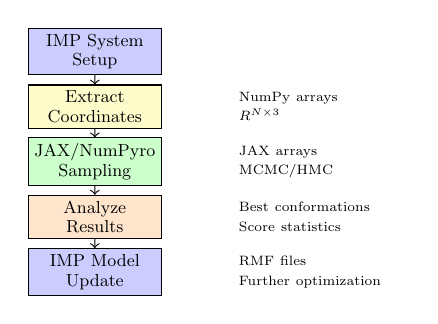
\begin{tikzpicture}[scale=0.7, transform shape]
    % Nodes
    \node[rectangle, draw, fill=blue!20, text width=2.2cm, text centered] (imp1) at (0,4) {IMP System\\Setup};
    
    \node[rectangle, draw, fill=yellow!20, text width=2.2cm, text centered] (extract) at (0,3) {Extract\\Coordinates};
    
    \node[rectangle, draw, fill=green!20, text width=2.2cm, text centered] (sample) at (0,2) {JAX/NumPyro\\Sampling};
    
    \node[rectangle, draw, fill=orange!20, text width=2.2cm, text centered] (analyze) at (0,1) {Analyze\\Results};
    
    \node[rectangle, draw, fill=blue!20, text width=2.2cm, text centered] (imp2) at (0,0) {IMP Model\\Update};
    
    % Arrows
    \draw[->] (imp1) -- (extract);
    \draw[->] (extract) -- (sample);
    \draw[->] (sample) -- (analyze);
    \draw[->] (analyze) -- (imp2);
    
    % Side annotations
    \node[right, text width=3cm] at (2.5,3) {\footnotesize NumPy arrays\\$\mathbb{R}^{N \times 3}$};
    \node[right, text width=3cm] at (2.5,2) {\footnotesize JAX arrays\\MCMC/HMC};
    \node[right, text width=3cm] at (2.5,1) {\footnotesize Best conformations\\Score statistics};
    \node[right, text width=3cm] at (2.5,0) {\footnotesize RMF files\\Further optimization};
\end{tikzpicture}

\vspace{0.3cm}
\textbf{Key Benefits:}
\begin{itemize}
    \item \alert{Enhanced sampling}: Beyond local minima
    \item \alert{Uncertainty quantification}: Conformational ensembles
    \item \alert{Seamless integration}: Native IMP formats
    \item \alert{Scalability}: GPU acceleration (when available)
\end{itemize}
\end{column}
\end{columns}
\end{frame}

%% SLIDE 6: Technical Challenges and Solutions
\begin{frame}{Technical Challenges \& Solutions}
\begin{columns}[T]
\begin{column}{0.5\textwidth}
\textbf{Major Challenges Encountered:}

\begin{enumerate}
    \item \alert{Array Conversion Errors}
    \begin{itemize}
        \item JAX tracers cannot be converted to NumPy
        \item Solution: Separate JAX and NumPy operations
    \end{itemize}
    
    \vspace{0.3cm}
    \item \alert{CUDA Compatibility Issues}
    \begin{itemize}
        \item CuDNN version mismatches
        \item Solution: Force CPU-only JAX execution
    \end{itemize}
    
    \vspace{0.3cm}
    \item \alert{Black-box Likelihood Problem}
    \begin{itemize}
        \item IMP's C++ backend not differentiable
        \item Solution: Hybrid approach or gradient-free samplers
    \end{itemize}
    
    \vspace{0.3cm}
    \item \alert{Scoring Function Adaptation}
    \begin{itemize}
        \item PMI restraints vs. raw IMP restraints
        \item Solution: Extract underlying IMP objects
    \end{itemize}
\end{enumerate}
\end{column}

\begin{column}{0.5\textwidth}
\textbf{Performance Optimizations:}

\begin{itemize}
    \item \alert{Adaptive Step Sizes}: Target 50\% acceptance rate
    \item \alert{Temperature Scheduling}: Better landscape exploration
    \item \alert{Batch Evaluation}: Process multiple configurations
    \item \alert{Smart Fallbacks}: Graceful degradation when methods fail
\end{itemize}

\vspace{0.5cm}
\textbf{Future Directions:}

\begin{itemize}
    \item \alert{Full JAX Implementation}: Rewrite key restraints in JAX
    \item \alert{GPU Acceleration}: Resolve CUDA compatibility
    \item \alert{Advanced Samplers}: Implement specialized MCMC for molecular systems
    \item \alert{Parallel Chains}: Multi-chain sampling for better convergence
\end{itemize}

\vspace{0.5cm}
\textbf{Code Structure:}
\begin{itemize}
    \item \alert{Modular Design}: Separate concerns (System, Scoring, Sampling)
    \item \alert{Error Handling}: Robust fallbacks at each step
    \item \alert{IMP Compatibility}: Maintains native IMP workflows
\end{itemize}
\end{column}
\end{columns}
\end{frame}



\end{document}